\documentclass[]{article}
\usepackage{lmodern}
\usepackage{amssymb,amsmath}
\usepackage{ifxetex,ifluatex}
\usepackage{fixltx2e} % provides \textsubscript
\ifnum 0\ifxetex 1\fi\ifluatex 1\fi=0 % if pdftex
  \usepackage[T1]{fontenc}
  \usepackage[utf8]{inputenc}
\else % if luatex or xelatex
  \ifxetex
    \usepackage{mathspec}
  \else
    \usepackage{fontspec}
  \fi
  \defaultfontfeatures{Ligatures=TeX,Scale=MatchLowercase}
\fi
% use upquote if available, for straight quotes in verbatim environments
\IfFileExists{upquote.sty}{\usepackage{upquote}}{}
% use microtype if available
\IfFileExists{microtype.sty}{%
\usepackage{microtype}
\UseMicrotypeSet[protrusion]{basicmath} % disable protrusion for tt fonts
}{}
\usepackage[margin=1in]{geometry}
\usepackage{hyperref}
\hypersetup{unicode=true,
            pdftitle={Homework 3},
            pdfauthor={Emorie Beck},
            pdfborder={0 0 0},
            breaklinks=true}
\urlstyle{same}  % don't use monospace font for urls
\usepackage{color}
\usepackage{fancyvrb}
\newcommand{\VerbBar}{|}
\newcommand{\VERB}{\Verb[commandchars=\\\{\}]}
\DefineVerbatimEnvironment{Highlighting}{Verbatim}{commandchars=\\\{\}}
% Add ',fontsize=\small' for more characters per line
\usepackage{framed}
\definecolor{shadecolor}{RGB}{248,248,248}
\newenvironment{Shaded}{\begin{snugshade}}{\end{snugshade}}
\newcommand{\KeywordTok}[1]{\textcolor[rgb]{0.13,0.29,0.53}{\textbf{#1}}}
\newcommand{\DataTypeTok}[1]{\textcolor[rgb]{0.13,0.29,0.53}{#1}}
\newcommand{\DecValTok}[1]{\textcolor[rgb]{0.00,0.00,0.81}{#1}}
\newcommand{\BaseNTok}[1]{\textcolor[rgb]{0.00,0.00,0.81}{#1}}
\newcommand{\FloatTok}[1]{\textcolor[rgb]{0.00,0.00,0.81}{#1}}
\newcommand{\ConstantTok}[1]{\textcolor[rgb]{0.00,0.00,0.00}{#1}}
\newcommand{\CharTok}[1]{\textcolor[rgb]{0.31,0.60,0.02}{#1}}
\newcommand{\SpecialCharTok}[1]{\textcolor[rgb]{0.00,0.00,0.00}{#1}}
\newcommand{\StringTok}[1]{\textcolor[rgb]{0.31,0.60,0.02}{#1}}
\newcommand{\VerbatimStringTok}[1]{\textcolor[rgb]{0.31,0.60,0.02}{#1}}
\newcommand{\SpecialStringTok}[1]{\textcolor[rgb]{0.31,0.60,0.02}{#1}}
\newcommand{\ImportTok}[1]{#1}
\newcommand{\CommentTok}[1]{\textcolor[rgb]{0.56,0.35,0.01}{\textit{#1}}}
\newcommand{\DocumentationTok}[1]{\textcolor[rgb]{0.56,0.35,0.01}{\textbf{\textit{#1}}}}
\newcommand{\AnnotationTok}[1]{\textcolor[rgb]{0.56,0.35,0.01}{\textbf{\textit{#1}}}}
\newcommand{\CommentVarTok}[1]{\textcolor[rgb]{0.56,0.35,0.01}{\textbf{\textit{#1}}}}
\newcommand{\OtherTok}[1]{\textcolor[rgb]{0.56,0.35,0.01}{#1}}
\newcommand{\FunctionTok}[1]{\textcolor[rgb]{0.00,0.00,0.00}{#1}}
\newcommand{\VariableTok}[1]{\textcolor[rgb]{0.00,0.00,0.00}{#1}}
\newcommand{\ControlFlowTok}[1]{\textcolor[rgb]{0.13,0.29,0.53}{\textbf{#1}}}
\newcommand{\OperatorTok}[1]{\textcolor[rgb]{0.81,0.36,0.00}{\textbf{#1}}}
\newcommand{\BuiltInTok}[1]{#1}
\newcommand{\ExtensionTok}[1]{#1}
\newcommand{\PreprocessorTok}[1]{\textcolor[rgb]{0.56,0.35,0.01}{\textit{#1}}}
\newcommand{\AttributeTok}[1]{\textcolor[rgb]{0.77,0.63,0.00}{#1}}
\newcommand{\RegionMarkerTok}[1]{#1}
\newcommand{\InformationTok}[1]{\textcolor[rgb]{0.56,0.35,0.01}{\textbf{\textit{#1}}}}
\newcommand{\WarningTok}[1]{\textcolor[rgb]{0.56,0.35,0.01}{\textbf{\textit{#1}}}}
\newcommand{\AlertTok}[1]{\textcolor[rgb]{0.94,0.16,0.16}{#1}}
\newcommand{\ErrorTok}[1]{\textcolor[rgb]{0.64,0.00,0.00}{\textbf{#1}}}
\newcommand{\NormalTok}[1]{#1}
\usepackage{graphicx,grffile}
\makeatletter
\def\maxwidth{\ifdim\Gin@nat@width>\linewidth\linewidth\else\Gin@nat@width\fi}
\def\maxheight{\ifdim\Gin@nat@height>\textheight\textheight\else\Gin@nat@height\fi}
\makeatother
% Scale images if necessary, so that they will not overflow the page
% margins by default, and it is still possible to overwrite the defaults
% using explicit options in \includegraphics[width, height, ...]{}
\setkeys{Gin}{width=\maxwidth,height=\maxheight,keepaspectratio}
\IfFileExists{parskip.sty}{%
\usepackage{parskip}
}{% else
\setlength{\parindent}{0pt}
\setlength{\parskip}{6pt plus 2pt minus 1pt}
}
\setlength{\emergencystretch}{3em}  % prevent overfull lines
\providecommand{\tightlist}{%
  \setlength{\itemsep}{0pt}\setlength{\parskip}{0pt}}
\setcounter{secnumdepth}{0}
% Redefines (sub)paragraphs to behave more like sections
\ifx\paragraph\undefined\else
\let\oldparagraph\paragraph
\renewcommand{\paragraph}[1]{\oldparagraph{#1}\mbox{}}
\fi
\ifx\subparagraph\undefined\else
\let\oldsubparagraph\subparagraph
\renewcommand{\subparagraph}[1]{\oldsubparagraph{#1}\mbox{}}
\fi

%%% Use protect on footnotes to avoid problems with footnotes in titles
\let\rmarkdownfootnote\footnote%
\def\footnote{\protect\rmarkdownfootnote}

%%% Change title format to be more compact
\usepackage{titling}

% Create subtitle command for use in maketitle
\newcommand{\subtitle}[1]{
  \posttitle{
    \begin{center}\large#1\end{center}
    }
}

\setlength{\droptitle}{-2em}
  \title{Homework 3}
  \pretitle{\vspace{\droptitle}\centering\huge}
  \posttitle{\par}
\subtitle{Psych 5068}
  \author{Emorie Beck}
  \preauthor{\centering\large\emph}
  \postauthor{\par}
  \predate{\centering\large\emph}
  \postdate{\par}
  \date{\today}

\usepackage{fancyhdr}
\usepackage{array}
\usepackage{longtable}
\usepackage{lscape}
\newcommand{\blandscape}{\begin{landscape}}
\newcommand{\elandscape}{\end{landscape}}
\usepackage{dcolumn}
\usepackage{bbm}
\usepackage{threeparttable}
\usepackage{booktabs}
\usepackage{expex}
\usepackage{rotating, graphicx}
\usepackage{tabulary}
\usepackage{algorithm}
\usepackage{multirow}
\usepackage{colortbl}
\usepackage{longtable}
\usepackage{array}
\usepackage{multirow}
\usepackage[table]{xcolor}
\usepackage{wrapfig}
\usepackage{float}
\usepackage{pdflscape}
\usepackage{tabu}
\usepackage{threeparttable}
\usepackage{booktabs}
\usepackage{longtable}
\usepackage{array}
\usepackage{multirow}
\usepackage[table]{xcolor}
\usepackage{wrapfig}
\usepackage{float}
\usepackage{colortbl}
\usepackage{pdflscape}
\usepackage{tabu}
\usepackage{threeparttable}
\usepackage[normalem]{ulem}

\begin{document}
\maketitle

{
\setcounter{tocdepth}{2}
\tableofcontents
}
\section{Workspace}\label{workspace}

\subsection{Packages}\label{packages}

\begin{Shaded}
\begin{Highlighting}[]
\KeywordTok{library}\NormalTok{(psych)}
\KeywordTok{library}\NormalTok{(lme4)}
\KeywordTok{library}\NormalTok{(knitr)}
\KeywordTok{library}\NormalTok{(kableExtra)}
\KeywordTok{library}\NormalTok{(plyr)}
\KeywordTok{library}\NormalTok{(tidyverse)}
\end{Highlighting}
\end{Shaded}

\subsection{Data}\label{data}

\begin{Shaded}
\begin{Highlighting}[]
\NormalTok{data_url <-}\StringTok{ "https://raw.githubusercontent.com/emoriebeck/homeworks/master/homework3/popularity_2(1).csv"}
\NormalTok{dat      <-}\StringTok{ }\KeywordTok{read.csv}\NormalTok{(}\KeywordTok{url}\NormalTok{(data_url)) }\OperatorTok\StringTok{ }\NormalTok{tbl_df }\OperatorTok
\StringTok{  }\KeywordTok{mutate}\NormalTok{(}\DataTypeTok{sex_c =} \KeywordTok{as.numeric}\NormalTok{(}\KeywordTok{scale}\NormalTok{(sex, }\DataTypeTok{scale =}\NormalTok{ F)),}
         \DataTypeTok{sex =} \KeywordTok{factor}\NormalTok{(sex, }\DataTypeTok{levels =} \DecValTok{0}\OperatorTok{:}\DecValTok{1}\NormalTok{, }\DataTypeTok{labels =} \KeywordTok{c}\NormalTok{(}\StringTok{"Male"}\NormalTok{, }\StringTok{"Female"}\NormalTok{)))}
\end{Highlighting}
\end{Shaded}

The popularity data include the teachers' ratings of the popularity of
the students in their classrooms. For this assignment, you will test
several hypotheses about the relationship between peer and teacher
popularity ratings, using the file: popularity\_2.csv. This file
contains the following variables:

sex: Male=0, Female=1 texp: Teacher's experience in years popular:
Average of other students' popularity ratings for the student, ranging
from 0 to 10 popteach: Teacher's popularity rating for the student,
ranging from 0 to 10

Conduct the following analyses:

\section{Question 1}\label{question-1}

\begin{enumerate}
\def\labelenumi{\arabic{enumi}.}
\tightlist
\item
  First, modify the data in the following ways:
\end{enumerate}

\subsection{Part A}\label{part-a}

Create the class average for teacher popularity ratings (call it
mean\_pop\_t).

\begin{Shaded}
\begin{Highlighting}[]
\NormalTok{dat <-}\StringTok{ }\NormalTok{dat }\OperatorTok\StringTok{ }\KeywordTok{group_by}\NormalTok{(class) }\OperatorTok\StringTok{ }\KeywordTok{mutate}\NormalTok{(}\DataTypeTok{mean_pop_t =} \KeywordTok{mean}\NormalTok{(popteach, }\DataTypeTok{na.rm =}\NormalTok{ T)) }\OperatorTok\StringTok{ }\KeywordTok{ungroup}\NormalTok{()}
\end{Highlighting}
\end{Shaded}

\subsection{Part B}\label{part-b}

Create a class-centered teacher popularity rating (call it popteach\_c).

\begin{Shaded}
\begin{Highlighting}[]
\NormalTok{dat <-}\StringTok{ }\NormalTok{dat }\OperatorTok\StringTok{ }\KeywordTok{mutate}\NormalTok{(}\DataTypeTok{popteach_c =}\NormalTok{ popteach }\OperatorTok{-}\StringTok{ }\NormalTok{mean_pop_t)}
\end{Highlighting}
\end{Shaded}

\subsection{Part C}\label{part-c}

Grand mean center the results of the calculation in (a). Call it
gmc\_mean\_pop\_t.

\begin{Shaded}
\begin{Highlighting}[]
\NormalTok{dat <-}\StringTok{ }\NormalTok{dat }\OperatorTok\StringTok{ }\KeywordTok{mutate}\NormalTok{(}\DataTypeTok{gmc_mean_pop_t =}\NormalTok{ mean_pop_t }\OperatorTok{-}\StringTok{ }\KeywordTok{mean}\NormalTok{(popteach, }\DataTypeTok{na.rm =}\NormalTok{ T)) }\OperatorTok\StringTok{ }\KeywordTok{ungroup}\NormalTok{()}
\end{Highlighting}
\end{Shaded}

\subsection{Part D}\label{part-d}

Create a grand-mean-centered version of texp called gmc\_texp. Include
the head( ) function to list the first 30 lines of the data frame to
show the results of the required calculations.

\begin{Shaded}
\begin{Highlighting}[]
\NormalTok{dat <-}\StringTok{ }\NormalTok{dat }\OperatorTok\StringTok{ }\KeywordTok{mutate}\NormalTok{(}\DataTypeTok{gmc_texp =} \KeywordTok{as.numeric}\NormalTok{(}\KeywordTok{scale}\NormalTok{(texp, }\DataTypeTok{scale =}\NormalTok{ F)))}

\KeywordTok{head}\NormalTok{(dat, }\DataTypeTok{n =} \DecValTok{30}\NormalTok{)}
\end{Highlighting}
\end{Shaded}

\begin{verbatim}
## # A tibble: 30 x 11
##    pupil class sex     texp popular popteach  sex_c mean_pop_t popteach_c
##    <int> <int> <fct>  <int>   <dbl>    <int>  <dbl>      <dbl>      <dbl>
##  1     1     1 Female    24    6.30        6  0.495       4.90     1.10  
##  2     2     1 Male      24    4.90        5 -0.505       4.90     0.1000
##  3     3     1 Female    24    5.30        6  0.495       4.90     1.10  
##  4     4     1 Female    24    4.70        5  0.495       4.90     0.1000
##  5     5     1 Female    24    6.00        6  0.495       4.90     1.10  
##  6     6     1 Male      24    4.70        5 -0.505       4.90     0.1000
##  7     7     1 Male      24    5.90        5 -0.505       4.90     0.1000
##  8     8     1 Male      24    4.20        5 -0.505       4.90     0.1000
##  9     9     1 Male      24    5.20        5 -0.505       4.90     0.1000
## 10    10     1 Male      24    3.90        3 -0.505       4.90    -1.90  
## # ... with 20 more rows, and 2 more variables: gmc_mean_pop_t <dbl>,
## #   gmc_texp <dbl>
\end{verbatim}

\section{Question 2}\label{question-2}

Then begin with the fully unconditional model for peer-rated popularity:

\[popular_{ij} = \beta_{0} + r_{ij}\] \[\beta_0 = \gamma_{00} + u_{0j}\]

Compare it to the following model that includes popteach\_c as a Level 1
predictor:

\[popular_{ij} = \beta_{0} + \beta_1 * popteach\_c_{ij} + r_{ij}\]
\[\beta_0 = \gamma_{00} + u_{0j}\] \[\beta_1 = \gamma_{10} + u_{1j}\]

\begin{Shaded}
\begin{Highlighting}[]
\NormalTok{mod0 <-}\StringTok{ }\KeywordTok{lmer}\NormalTok{(popular }\OperatorTok{~}\StringTok{ }\DecValTok{1}          \OperatorTok{+}\StringTok{ }\NormalTok{(}\DecValTok{1}\OperatorTok{|}\NormalTok{class), }\DataTypeTok{data =}\NormalTok{ dat)}
\NormalTok{mod1 <-}\StringTok{ }\KeywordTok{lmer}\NormalTok{(popular }\OperatorTok{~}\StringTok{ }\NormalTok{popteach_c }\OperatorTok{+}\StringTok{ }\NormalTok{(popteach_c}\OperatorTok{|}\NormalTok{class), }\DataTypeTok{data =}\NormalTok{ dat)}

\KeywordTok{source}\NormalTok{(}\StringTok{"https://raw.githubusercontent.com/emoriebeck/homeworks/master/table_fun.R"}\NormalTok{)}

\NormalTok{tab0 <-}\StringTok{ }\KeywordTok{table_fun}\NormalTok{(mod0) }\OperatorTok\StringTok{ }\KeywordTok{mutate}\NormalTok{(}\DataTypeTok{model =} \StringTok{"unconditional"}\NormalTok{) }
\NormalTok{tab1 <-}\StringTok{ }\KeywordTok{table_fun}\NormalTok{(mod1) }\OperatorTok\StringTok{ }\KeywordTok{mutate}\NormalTok{(}\DataTypeTok{model =} \StringTok{"conditional"}\NormalTok{)}

\KeywordTok{options}\NormalTok{(}\DataTypeTok{knitr.kable.NA =} \StringTok{''}\NormalTok{)}
\NormalTok{tab0 }\OperatorTok\StringTok{ }\KeywordTok{full_join}\NormalTok{(tab1) }\OperatorTok
\StringTok{  }\KeywordTok{mutate}\NormalTok{(}\DataTypeTok{term =} \KeywordTok{str_replace_all}\NormalTok{(term, }\StringTok{"}\CharTok{\textbackslash{}\textbackslash{}}\StringTok{_"}\NormalTok{, }\StringTok{"}\CharTok{\textbackslash{}\textbackslash{}\textbackslash{}\textbackslash{}}\StringTok{_"}\NormalTok{)) }\OperatorTok
\StringTok{  }\KeywordTok{gather}\NormalTok{(}\DataTypeTok{key =}\NormalTok{ est, }\DataTypeTok{value =}\NormalTok{ value, b, CI) }\OperatorTok
\StringTok{  }\KeywordTok{unite}\NormalTok{(tmp, model, est, }\DataTypeTok{sep =} \StringTok{"."}\NormalTok{) }\OperatorTok
\StringTok{  }\KeywordTok{mutate}\NormalTok{(}\DataTypeTok{type =} \KeywordTok{factor}\NormalTok{(type, }\DataTypeTok{levels =} \KeywordTok{c}\NormalTok{(}\StringTok{"Fixed Parts"}\NormalTok{, }\StringTok{"Random Parts"}\NormalTok{, }\StringTok{"Model Terms"}\NormalTok{))) }\OperatorTok
\StringTok{  }\KeywordTok{spread}\NormalTok{(}\DataTypeTok{key =}\NormalTok{ tmp, }\DataTypeTok{value =}\NormalTok{ value) }\OperatorTok
\StringTok{  }\KeywordTok{select}\NormalTok{(term, }\KeywordTok{contains}\NormalTok{(}\StringTok{"uncond"}\NormalTok{), }\KeywordTok{contains}\NormalTok{(}\StringTok{"cond"}\NormalTok{)) }\OperatorTok
\StringTok{  }\KeywordTok{kable}\NormalTok{(., }\StringTok{"latex"}\NormalTok{, }\DataTypeTok{booktabs =}\NormalTok{ T, }\DataTypeTok{escape =}\NormalTok{ F,}
        \DataTypeTok{col.names =} \KeywordTok{c}\NormalTok{(}\StringTok{"Term"}\NormalTok{, }\StringTok{"b"}\NormalTok{, }\StringTok{"CI"}\NormalTok{, }\StringTok{"b"}\NormalTok{, }\StringTok{"CI"}\NormalTok{)) }\OperatorTok
\StringTok{  }\KeywordTok{kable_styling}\NormalTok{(}\DataTypeTok{full_width =}\NormalTok{ F) }\OperatorTok
\StringTok{  }\KeywordTok{column_spec}\NormalTok{(}\DecValTok{2}\OperatorTok{:}\DecValTok{5}\NormalTok{, }\DataTypeTok{width =} \StringTok{"2cm"}\NormalTok{) }\OperatorTok
\StringTok{  }\KeywordTok{group_rows}\NormalTok{(}\StringTok{"Fixed Parts"}\NormalTok{,}\DecValTok{1}\NormalTok{,}\DecValTok{2}\NormalTok{) }\OperatorTok
\StringTok{  }\KeywordTok{group_rows}\NormalTok{(}\StringTok{"Random Parts"}\NormalTok{,}\DecValTok{3}\NormalTok{,}\DecValTok{4}\NormalTok{) }\OperatorTok
\StringTok{  }\KeywordTok{group_rows}\NormalTok{(}\StringTok{"Model Terms"}\NormalTok{,}\DecValTok{5}\NormalTok{,}\DecValTok{6}\NormalTok{) }\OperatorTok
\StringTok{  }\KeywordTok{add_header_above}\NormalTok{(}\KeywordTok{c}\NormalTok{(}\StringTok{" "}\NormalTok{ =}\StringTok{ }\DecValTok{1}\NormalTok{, }\StringTok{"Unconditional"}\NormalTok{ =}\StringTok{ }\DecValTok{2}\NormalTok{, }\StringTok{"Conditional"}\NormalTok{ =}\StringTok{ }\DecValTok{2}\NormalTok{))}
\end{Highlighting}
\end{Shaded}

\begin{table}[H]
\centering
\begin{tabular}{l>{\raggedright\arraybackslash}p{2cm}>{\raggedright\arraybackslash}p{2cm}>{\raggedright\arraybackslash}p{2cm}>{\raggedright\arraybackslash}p{2cm}}
\toprule
\multicolumn{1}{c}{ } & \multicolumn{2}{c}{Unconditional} & \multicolumn{2}{c}{Conditional} \\
\cmidrule(l{2pt}r{2pt}){2-3} \cmidrule(l{2pt}r{2pt}){4-5}
Term & b & CI & b & CI\\
\midrule
\addlinespace[0.3em]
\multicolumn{5}{l}{\textbf{Fixed Parts}}\\
\hspace{1em}(Intercept) & 5.08 & [4.92, 5.18] & 5.08 & [4.99, 5.13]\\
\hspace{1em}popteach\_c &  &  & 0.73 & [0.71, 0.76]\\
\addlinespace[0.3em]
\multicolumn{5}{l}{\textbf{Random Parts}}\\
\hspace{1em}$\tau\_{00}$ & 0.70 & [0.49, 0.95] & 0.74 & [0.61, 0.96]\\
\hspace{1em}$\tau\_{11}$ &  &  & 0.00 & [0.00, 0.01]\\
$R^2\_c$ & 0.36 &  & 0.73 & \\
$R^2\_m$ & 0.00 &  & 0.34 & \\
\bottomrule
\end{tabular}
\end{table}

\subsection{Part A}\label{part-a-1}

Are peer-reports and teacher-reports significantly related? Yes, a one
unit increase in teacher ratings of popularity is associated with a
\(0.73\), 95\% CI \([0.71, 0.76]\).

\subsection{Part B}\label{part-b-1}

How much variance in the Level 1 model is accounted for by teacher
popularity ratings?

\begin{Shaded}
\begin{Highlighting}[]
\NormalTok{vexpL1 <-}\StringTok{ }\NormalTok{(}\KeywordTok{sigma}\NormalTok{(mod0)}\OperatorTok{^}\DecValTok{2} \OperatorTok{-}\StringTok{ }\KeywordTok{sigma}\NormalTok{(mod1)}\OperatorTok{^}\DecValTok{2}\NormalTok{)}\OperatorTok{/}\KeywordTok{sigma}\NormalTok{(mod0)}\OperatorTok{^}\DecValTok{2}
\end{Highlighting}
\end{Shaded}

\(58\)\% of the variance in the Level 1 model is accounted for by
teacher popularity ratings.

\section{Question 3}\label{question-3}

Now test two hypotheses about the ability of teachers as judges of their
students' popularity.

To test these hypotheses, analyze the following model:

\[popular_{ij} = \beta_{0} + \beta_1 * popteach\_c_{ij} + r_{ij}\]
\[\beta_0 = \gamma_{00} + \gamma_{01}*gmc\_texp_j + \gamma_{02}*gmc\_mean\_pop\_t_j + u_{0j}\]\\
\[\beta_1 = \gamma_{10} + \gamma_{11}*gmc\_texp_j + \gamma_{12}*gmc\_mean\_pop\_t_j + u_{1j}\]

\begin{Shaded}
\begin{Highlighting}[]
\NormalTok{mod2 <-}\StringTok{ }\KeywordTok{lmer}\NormalTok{(popular }\OperatorTok{~}\StringTok{ }\NormalTok{popteach_c }\OperatorTok{+}\StringTok{ }\NormalTok{gmc_texp }\OperatorTok{*}\StringTok{ }\NormalTok{popteach_c }\OperatorTok{+}\StringTok{ }\NormalTok{gmc_mean_pop_t }\OperatorTok{*}\StringTok{ }\NormalTok{popteach_c }\OperatorTok{+}\StringTok{ }\NormalTok{(popteach_c }\OperatorTok{|}\StringTok{ }\NormalTok{class), }\DataTypeTok{data =}\NormalTok{ dat)}
\NormalTok{tab2 <-}\StringTok{ }\KeywordTok{table_fun}\NormalTok{(mod2)}

\NormalTok{tab2 }\OperatorTok\StringTok{ }\KeywordTok{select}\NormalTok{(}\OperatorTok{-}\NormalTok{type) }\OperatorTok
\StringTok{  }\KeywordTok{mutate}\NormalTok{(}\DataTypeTok{term =} \KeywordTok{str_replace_all}\NormalTok{(term, }\StringTok{"}\CharTok{\textbackslash{}\textbackslash{}}\StringTok{_"}\NormalTok{, }\StringTok{"}\CharTok{\textbackslash{}\textbackslash{}\textbackslash{}\textbackslash{}}\StringTok{_"}\NormalTok{)) }\OperatorTok
\StringTok{  }\KeywordTok{kable}\NormalTok{(., }\StringTok{"latex"}\NormalTok{, }\DataTypeTok{booktabs =}\NormalTok{ T, }\DataTypeTok{escape =}\NormalTok{ F,}
        \DataTypeTok{col.names =} \KeywordTok{c}\NormalTok{(}\StringTok{"Term"}\NormalTok{, }\StringTok{"b"}\NormalTok{, }\StringTok{"CI"}\NormalTok{)) }\OperatorTok
\StringTok{  }\KeywordTok{kable_styling}\NormalTok{(}\DataTypeTok{full_width =}\NormalTok{ F) }\OperatorTok
\StringTok{  }\KeywordTok{column_spec}\NormalTok{(}\DecValTok{2}\OperatorTok{:}\DecValTok{3}\NormalTok{, }\DataTypeTok{width =} \StringTok{"2cm"}\NormalTok{) }\OperatorTok
\StringTok{  }\KeywordTok{group_rows}\NormalTok{(}\StringTok{"Fixed Parts"}\NormalTok{,}\DecValTok{1}\NormalTok{,}\DecValTok{6}\NormalTok{) }\OperatorTok
\StringTok{  }\KeywordTok{group_rows}\NormalTok{(}\StringTok{"Random Parts"}\NormalTok{,}\DecValTok{7}\NormalTok{,}\DecValTok{8}\NormalTok{) }\OperatorTok
\StringTok{  }\KeywordTok{group_rows}\NormalTok{(}\StringTok{"Model Terms"}\NormalTok{,}\DecValTok{9}\NormalTok{,}\DecValTok{10}\NormalTok{) }\OperatorTok
\StringTok{  }\KeywordTok{add_header_above}\NormalTok{(}\KeywordTok{c}\NormalTok{(}\StringTok{" "}\NormalTok{ =}\StringTok{ }\DecValTok{1}\NormalTok{, }\StringTok{"Popularity"}\NormalTok{ =}\StringTok{ }\DecValTok{2}\NormalTok{))}
\end{Highlighting}
\end{Shaded}

\begin{table}[H]
\centering
\begin{tabular}{l>{\raggedright\arraybackslash}p{2cm}>{\raggedright\arraybackslash}p{2cm}}
\toprule
\multicolumn{1}{c}{ } & \multicolumn{2}{c}{Popularity} \\
\cmidrule(l{2pt}r{2pt}){2-3}
Term & b & CI\\
\midrule
\addlinespace[0.3em]
\multicolumn{3}{l}{\textbf{Fixed Parts}}\\
\hspace{1em}(Intercept) & 5.08 & [5.06, 5.10]\\
\hspace{1em}popteach\_c & 0.72 & [0.69, 0.76]\\
\hspace{1em}gmc\_texp & 0.00 & [-0.00, 0.01]\\
\hspace{1em}gmc\_mean\_pop\_t & 0.98 & [0.95, 1.01]\\
\hspace{1em}popteach\_c:gmc\_texp & -0.01 & [-0.01, -0.00]\\
\hspace{1em}popteach\_c:gmc\_mean\_pop\_t & -0.01 & [-0.02, 0.04]\\
\addlinespace[0.3em]
\multicolumn{3}{l}{\textbf{Random Parts}}\\
\hspace{1em}$\tau\_{00}$ & 0.00 & [0.00, 0.01]\\
\hspace{1em}$\tau\_{11}$ & 0.00 & [0.00, 0.01]\\
$R^2\_m$ & 0.73 & \\
$R^2\_c$ & 0.73 & \\
\bottomrule
\end{tabular}
\end{table}

\subsection{Part A}\label{part-a-2}

Teachers with more experience are better judges of student popularity.
Teachers with more experience are worse judges of popularity,
\(\gamma_{11} = -0.01\), 95\% CI \([-0.01, -0.00]\).

\subsection{Part B}\label{part-b-2}

It is more difficult to judge student popularity when the mean
popularity of the class (as rated by teachers) is high than when it is
low.\\
It is not more difficult to judge student popularity when the mean
popularity is high v. low, \(\gamma_{12} = -0.01\), 95\% CI
\([-0.02, 0.04]\).

\subsection{Part C}\label{part-c-1}

Illustrate the cross-level interaction, \(\gamma_{11}\).

\begin{Shaded}
\begin{Highlighting}[]
\CommentTok{# get SD from unconditional model}
\NormalTok{mod.pt0 <-}\StringTok{ }\KeywordTok{lmer}\NormalTok{(popteach_c }\OperatorTok{~}\StringTok{ }\DecValTok{1} \OperatorTok{+}\StringTok{ }\NormalTok{(}\DecValTok{1} \OperatorTok{|}\StringTok{ }\NormalTok{class), }\DataTypeTok{data =}\NormalTok{ dat) }
\NormalTok{sd.pt0  <-}\StringTok{ }\KeywordTok{sigma}\NormalTok{(mod.pt0)}
\NormalTok{sd.te   <-}\StringTok{ }\KeywordTok{sd}\NormalTok{(dat}\OperatorTok{$}\NormalTok{texp)}

\NormalTok{mod.pt1 <-}\StringTok{ }\KeywordTok{lmer}\NormalTok{(popteach_c }\OperatorTok{~}\StringTok{ }\DecValTok{1} \OperatorTok{+}\StringTok{ }\NormalTok{gmc_texp }\OperatorTok{+}\StringTok{ }\NormalTok{gmc_mean_pop_t }\OperatorTok{+}\StringTok{ }\NormalTok{(}\DecValTok{1} \OperatorTok{|}\StringTok{ }\NormalTok{class), }\DataTypeTok{data =}\NormalTok{ dat) }

\NormalTok{te.inc.}\DecValTok{1}\NormalTok{ <-}\StringTok{ }\NormalTok{sd.te }\OperatorTok{*}\StringTok{ }\KeywordTok{fixef}\NormalTok{(mod.pt1)[}\StringTok{"gmc_texp"}\NormalTok{] }

\KeywordTok{tibble}\NormalTok{(}
  \DataTypeTok{class=}\DecValTok{1}\NormalTok{, }
  \DataTypeTok{popteach_c =} \KeywordTok{seq}\NormalTok{(}\OperatorTok{-}\DecValTok{1}\OperatorTok{*}\NormalTok{te.inc.}\DecValTok{1} \OperatorTok{-}\StringTok{ }\NormalTok{sd.pt0,}\OperatorTok{-}\NormalTok{te.inc.}\DecValTok{1} \OperatorTok{+}\StringTok{ }\NormalTok{sd.pt0, }\DataTypeTok{by =}\NormalTok{ sd.pt0), }
  \DataTypeTok{gmc_texp =} \OperatorTok{-}\NormalTok{sd.te, }
  \DataTypeTok{gmc_mean_pop_t =} \KeywordTok{mean}\NormalTok{(dat}\OperatorTok{$}\NormalTok{gmc_mean_pop_t),}
  \DataTypeTok{level =} \StringTok{"-1 SD"}
\NormalTok{  ) }\OperatorTok\StringTok{ }\KeywordTok{full_join}\NormalTok{(}
\KeywordTok{tibble}\NormalTok{(}
  \DataTypeTok{class=}\DecValTok{1}\NormalTok{, }
  \DataTypeTok{popteach_c =} \KeywordTok{seq}\NormalTok{(}\OperatorTok{-}\NormalTok{sd.pt0,sd.pt0, }\DataTypeTok{by =}\NormalTok{ sd.pt0), }
  \DataTypeTok{gmc_texp =} \DecValTok{0}\NormalTok{, }
  \DataTypeTok{gmc_mean_pop_t =} \KeywordTok{mean}\NormalTok{(dat}\OperatorTok{$}\NormalTok{gmc_mean_pop_t),}
  \DataTypeTok{level =} \StringTok{"0 SD"}
\NormalTok{)) }\OperatorTok\StringTok{ }\KeywordTok{full_join}\NormalTok{(}
\KeywordTok{tibble}\NormalTok{(}
  \DataTypeTok{class=}\DecValTok{1}\NormalTok{, }
  \DataTypeTok{popteach_c =} \KeywordTok{seq}\NormalTok{(te.inc.}\DecValTok{1} \OperatorTok{-}\StringTok{ }\NormalTok{sd.pt0,te.inc.}\DecValTok{1} \OperatorTok{+}\StringTok{ }\NormalTok{sd.pt0, }\DataTypeTok{by =}\NormalTok{ sd.pt0), }
  \DataTypeTok{gmc_texp =}\NormalTok{ sd.te, }
  \DataTypeTok{gmc_mean_pop_t =} \KeywordTok{mean}\NormalTok{(dat}\OperatorTok{$}\NormalTok{gmc_mean_pop_t),}
  \DataTypeTok{level =} \StringTok{"+1 SD"}
\NormalTok{)) }\OperatorTok
\StringTok{  }\KeywordTok{mutate}\NormalTok{(}\DataTypeTok{pred =} \KeywordTok{predict}\NormalTok{(mod2, .),}
         \DataTypeTok{level =} \KeywordTok{factor}\NormalTok{(level, }\KeywordTok{c}\NormalTok{(}\StringTok{"-1 SD"}\NormalTok{, }\StringTok{"0 SD"}\NormalTok{, }\StringTok{"+1 SD"}\NormalTok{))) }\OperatorTok
\StringTok{  }\KeywordTok{ggplot}\NormalTok{(}\KeywordTok{aes}\NormalTok{(}\DataTypeTok{x =}\NormalTok{ popteach_c, }\DataTypeTok{y =}\NormalTok{ pred, }\DataTypeTok{color =}\NormalTok{ level)) }\OperatorTok{+}
\StringTok{  }\KeywordTok{geom_line}\NormalTok{(}\DataTypeTok{size =} \FloatTok{1.5}\NormalTok{) }\OperatorTok{+}
\StringTok{  }\KeywordTok{theme_classic}\NormalTok{() }\OperatorTok{+}
\StringTok{  }\KeywordTok{theme}\NormalTok{(}\DataTypeTok{legend.position =} \StringTok{"bottom"}\NormalTok{,}
        \DataTypeTok{axis.text =} \KeywordTok{element_text}\NormalTok{(}\DataTypeTok{face =} \StringTok{"bold"}\NormalTok{, }\DataTypeTok{size =} \KeywordTok{rel}\NormalTok{(}\FloatTok{1.2}\NormalTok{)),}
        \DataTypeTok{axis.title =} \KeywordTok{element_text}\NormalTok{(}\DataTypeTok{face =} \StringTok{"bold"}\NormalTok{, }\DataTypeTok{size =} \KeywordTok{rel}\NormalTok{(}\FloatTok{1.2}\NormalTok{)),}
        \DataTypeTok{legend.text =} \KeywordTok{element_text}\NormalTok{(}\DataTypeTok{face =} \StringTok{"bold"}\NormalTok{, }\DataTypeTok{size =} \KeywordTok{rel}\NormalTok{(}\FloatTok{1.2}\NormalTok{)),}
        \DataTypeTok{legend.title =} \KeywordTok{element_text}\NormalTok{(}\DataTypeTok{face =} \StringTok{"bold"}\NormalTok{, }\DataTypeTok{size =} \KeywordTok{rel}\NormalTok{(}\FloatTok{1.2}\NormalTok{)))}
\end{Highlighting}
\end{Shaded}

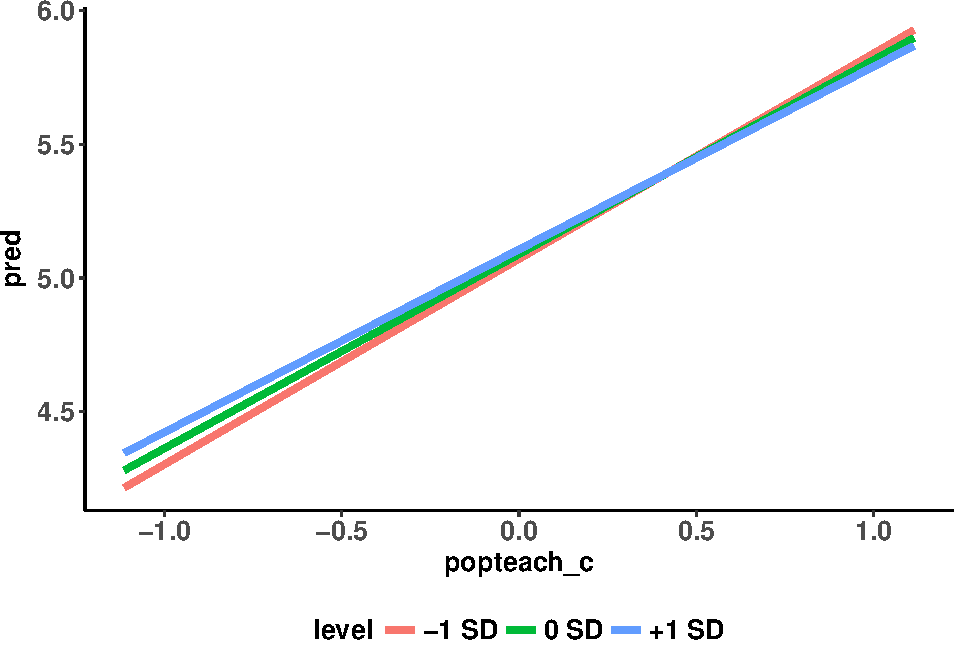
\includegraphics{Beck_HW_3_files/figure-latex/Q2c-1.pdf}

\subsection{Part D}\label{part-d-1}

Illustrate the cross-level interaction, \(\gamma_{12}\).

\begin{Shaded}
\begin{Highlighting}[]
\CommentTok{# get SD from unconditional model}
\NormalTok{mod.pt0 <-}\StringTok{ }\KeywordTok{lmer}\NormalTok{(popteach_c }\OperatorTok{~}\StringTok{ }\DecValTok{1} \OperatorTok{+}\StringTok{ }\NormalTok{(}\DecValTok{1} \OperatorTok{|}\StringTok{ }\NormalTok{class), }\DataTypeTok{data =}\NormalTok{ dat) }
\NormalTok{sd.pt0  <-}\StringTok{ }\KeywordTok{sigma}\NormalTok{(mod.pt0)}
\NormalTok{sd.mtp  <-}\StringTok{ }\KeywordTok{sd}\NormalTok{(dat}\OperatorTok{$}\NormalTok{gmc_mean_pop_t)  }

\NormalTok{mod.pt1 <-}\StringTok{ }\KeywordTok{lmer}\NormalTok{(popteach_c }\OperatorTok{~}\StringTok{ }\DecValTok{1} \OperatorTok{+}\StringTok{ }\NormalTok{gmc_texp }\OperatorTok{+}\StringTok{ }\NormalTok{gmc_mean_pop_t }\OperatorTok{+}\StringTok{ }\NormalTok{(}\DecValTok{1} \OperatorTok{|}\StringTok{ }\NormalTok{class), }\DataTypeTok{data =}\NormalTok{ dat) }

\NormalTok{te.inc.}\DecValTok{1}\NormalTok{ <-}\StringTok{ }\NormalTok{sd.mtp }\OperatorTok{*}\StringTok{ }\KeywordTok{fixef}\NormalTok{(mod.pt1)[}\StringTok{"gmc_mean_pop_t"}\NormalTok{] }

\KeywordTok{tibble}\NormalTok{(}
  \DataTypeTok{class=}\DecValTok{1}\NormalTok{, }
  \DataTypeTok{popteach_c =} \KeywordTok{seq}\NormalTok{(te.inc.}\DecValTok{1} \OperatorTok{-}\StringTok{ }\NormalTok{sd.pt0,te.inc.}\DecValTok{1} \OperatorTok{+}\StringTok{ }\NormalTok{sd.pt0, }\DataTypeTok{by =}\NormalTok{ sd.pt0), }
  \DataTypeTok{gmc_texp =} \KeywordTok{mean}\NormalTok{(dat}\OperatorTok{$}\NormalTok{gmc_texp), }
  \DataTypeTok{gmc_mean_pop_t =} \OperatorTok{-}\NormalTok{sd.mtp,}
  \DataTypeTok{level =} \StringTok{"-1 SD"}
\NormalTok{  ) }\OperatorTok\StringTok{ }\KeywordTok{full_join}\NormalTok{(}
\KeywordTok{tibble}\NormalTok{(}
  \DataTypeTok{class=}\DecValTok{1}\NormalTok{, }
  \DataTypeTok{popteach_c =} \KeywordTok{seq}\NormalTok{(}\OperatorTok{-}\NormalTok{sd.pt0, sd.pt0, }\DataTypeTok{by =}\NormalTok{ sd.pt0), }
  \DataTypeTok{gmc_texp =} \KeywordTok{mean}\NormalTok{(dat}\OperatorTok{$}\NormalTok{gmc_texp), }
  \DataTypeTok{gmc_mean_pop_t =} \DecValTok{0}\NormalTok{,}
  \DataTypeTok{level =} \StringTok{"0 SD"}
\NormalTok{)) }\OperatorTok\StringTok{ }\KeywordTok{full_join}\NormalTok{(}
\KeywordTok{tibble}\NormalTok{(}
  \DataTypeTok{class=}\DecValTok{1}\NormalTok{, }
  \DataTypeTok{popteach_c =} \KeywordTok{seq}\NormalTok{(}\OperatorTok{-}\NormalTok{te.inc.}\DecValTok{1} \OperatorTok{-}\StringTok{ }\NormalTok{sd.pt0,}\OperatorTok{-}\NormalTok{te.inc.}\DecValTok{1} \OperatorTok{+}\StringTok{ }\NormalTok{sd.pt0, }\DataTypeTok{by =}\NormalTok{ sd.pt0), }
  \DataTypeTok{gmc_texp =} \KeywordTok{mean}\NormalTok{(dat}\OperatorTok{$}\NormalTok{gmc_texp), }
  \DataTypeTok{gmc_mean_pop_t =}\NormalTok{ sd.mtp,}
  \DataTypeTok{level =} \StringTok{"+1 SD"}
\NormalTok{)) }\OperatorTok
\StringTok{  }\KeywordTok{mutate}\NormalTok{(}\DataTypeTok{pred =} \KeywordTok{predict}\NormalTok{(mod2, .),}
         \DataTypeTok{level =} \KeywordTok{factor}\NormalTok{(level, }\KeywordTok{c}\NormalTok{(}\StringTok{"-1 SD"}\NormalTok{, }\StringTok{"0 SD"}\NormalTok{, }\StringTok{"+1 SD"}\NormalTok{))) }\OperatorTok
\StringTok{  }\KeywordTok{ggplot}\NormalTok{(}\KeywordTok{aes}\NormalTok{(}\DataTypeTok{x =}\NormalTok{ popteach_c, }\DataTypeTok{y =}\NormalTok{ pred, }\DataTypeTok{color =}\NormalTok{ level)) }\OperatorTok{+}
\StringTok{  }\KeywordTok{geom_line}\NormalTok{(}\DataTypeTok{size =} \FloatTok{1.5}\NormalTok{) }\OperatorTok{+}
\StringTok{  }\KeywordTok{theme_classic}\NormalTok{() }\OperatorTok{+}
\StringTok{  }\KeywordTok{theme}\NormalTok{(}\DataTypeTok{legend.position =} \StringTok{"bottom"}\NormalTok{,}
        \DataTypeTok{axis.text =} \KeywordTok{element_text}\NormalTok{(}\DataTypeTok{face =} \StringTok{"bold"}\NormalTok{, }\DataTypeTok{size =} \KeywordTok{rel}\NormalTok{(}\FloatTok{1.2}\NormalTok{)),}
        \DataTypeTok{axis.title =} \KeywordTok{element_text}\NormalTok{(}\DataTypeTok{face =} \StringTok{"bold"}\NormalTok{, }\DataTypeTok{size =} \KeywordTok{rel}\NormalTok{(}\FloatTok{1.2}\NormalTok{)),}
        \DataTypeTok{legend.text =} \KeywordTok{element_text}\NormalTok{(}\DataTypeTok{face =} \StringTok{"bold"}\NormalTok{, }\DataTypeTok{size =} \KeywordTok{rel}\NormalTok{(}\FloatTok{1.2}\NormalTok{)),}
        \DataTypeTok{legend.title =} \KeywordTok{element_text}\NormalTok{(}\DataTypeTok{face =} \StringTok{"bold"}\NormalTok{, }\DataTypeTok{size =} \KeywordTok{rel}\NormalTok{(}\FloatTok{1.2}\NormalTok{)))}
\end{Highlighting}
\end{Shaded}

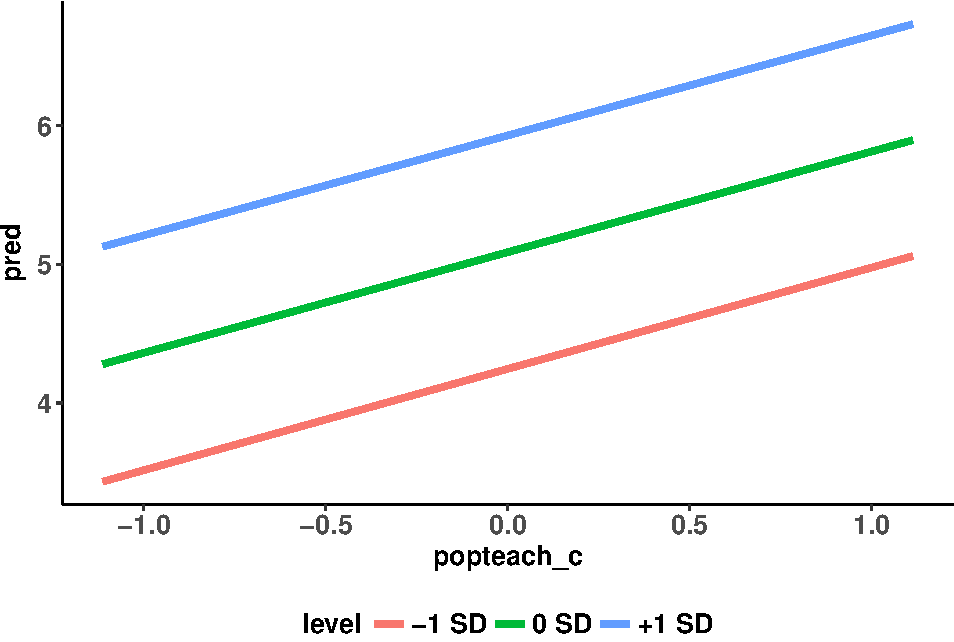
\includegraphics{Beck_HW_3_files/figure-latex/Q2d-1.pdf}

For (c) and (d) illustrate the interactions using a method of your
choosing. If you treat the continuous predictors as discrete for the
purpose of graphing, define ``low'' and ``high'' as + 1 standard
deviation from the grand mean. Remember that the simple standard
deviation taken across the entire data set may not be the best indicator
of variability for Level 1 predictors. Note also that displaying the
interactions most accurately involves accounting for the possible
relationship between teacher popularity ratings and teacher experience
and the possible relationship between teacher popularity ratings and
classroom mean teacher-rated popularity. A separate document (Additional
advice on figures for Homework 3) describes how to approach this if you
want to give it a go. Simpler figures (without any such adjustments) are
acceptable for this homework assignment.

\section{Question 4}\label{question-4}

Now test the hypothesis that it is more difficult for teachers to judge
the popularity of boys than to judge the popularity of girls. If true,
this would manifest itself in the form of a Teacher Rating x Sex of
Student interaction---the relationship of teacher ratings to peer
ratings would be different for male and female students. Test the
following model:

\[popular_{ij} = \beta_{0} + \beta_1*sex\_c_{ij}+ \beta_2 * popteach\_c_{ij} + \beta_3 * (sex\_c_{ij} : popteach\_c_{ij}) + r_{ij}\]
\[\beta_0 = \gamma_{00} + u_{0j}\] \[\beta_1 = \gamma_{10} + u_{1j}\]
\[\beta_2 = \gamma_{20} + u_{2j}\] \[\beta_3 = \gamma_{30} + u_{3j}\]

\begin{Shaded}
\begin{Highlighting}[]
\NormalTok{mod3 <-}\StringTok{ }\KeywordTok{lmer}\NormalTok{(popular }\OperatorTok{~}\StringTok{ }\NormalTok{sex_c }\OperatorTok{*}\StringTok{ }\NormalTok{popteach_c }\OperatorTok{+}\StringTok{ }\NormalTok{(sex_c}\OperatorTok{*}\NormalTok{popteach_c}\OperatorTok{|}\NormalTok{class), }\DataTypeTok{data =}\NormalTok{ dat)}
\NormalTok{tab3 <-}\StringTok{ }\KeywordTok{table_fun}\NormalTok{(mod3)}
\end{Highlighting}
\end{Shaded}

\subsection{Part A}\label{part-a-3}

Compared to the fully unconditional model, how much Level 1 variance is
accounted for by all Level 1 predictors?

\begin{Shaded}
\begin{Highlighting}[]
\NormalTok{vexpL1.4a <-}\StringTok{ }\NormalTok{(}\KeywordTok{sigma}\NormalTok{(mod0)}\OperatorTok{^}\DecValTok{2} \OperatorTok{-}\StringTok{ }\KeywordTok{sigma}\NormalTok{(mod3)}\OperatorTok{^}\DecValTok{2}\NormalTok{)}\OperatorTok{/}\KeywordTok{sigma}\NormalTok{(mod0)}\OperatorTok{^}\DecValTok{2}
\end{Highlighting}
\end{Shaded}

\(62\)\% of the variance in the Level 1 model is accounted for by all
predictors.

\subsection{Part B}\label{part-b-3}

How much is attributable to the addition of the sex main effect and the
interaction?

\begin{Shaded}
\begin{Highlighting}[]
\NormalTok{vexpL1.4b <-}\StringTok{ }\NormalTok{(}\KeywordTok{sigma}\NormalTok{(mod1)}\OperatorTok{^}\DecValTok{2} \OperatorTok{-}\StringTok{ }\KeywordTok{sigma}\NormalTok{(mod3)}\OperatorTok{^}\DecValTok{2}\NormalTok{)}\OperatorTok{/}\KeywordTok{sigma}\NormalTok{(mod1)}\OperatorTok{^}\DecValTok{2}
\end{Highlighting}
\end{Shaded}

\(11\)\% of the variance in the Level 1 model is accounted for by all
predictors.

\subsection{Part C}\label{part-c-2}

Is there support for the hypothesis? We cannot conclude that it is more
difficult for teachers to judge the popularity of boys than to judge the
popularity of girls, \(\gamma_{30} = 0.03\), 95\% CI \([-0.00, 0.07]\).

\subsection{Part D}\label{part-d-2}

Illustrate the interaction in this model.

\begin{Shaded}
\begin{Highlighting}[]
\KeywordTok{crossing}\NormalTok{(}\DataTypeTok{sex_c =} \KeywordTok{unique}\NormalTok{(dat}\OperatorTok{$}\NormalTok{sex_c),}
         \DataTypeTok{popteach_c =} \KeywordTok{seq}\NormalTok{(}\KeywordTok{min}\NormalTok{(dat}\OperatorTok{$}\NormalTok{popteach_c,}\DataTypeTok{na.rm =}\NormalTok{T), }\KeywordTok{max}\NormalTok{(dat}\OperatorTok{$}\NormalTok{popteach_c, }\DataTypeTok{na.rm =}\NormalTok{ T), .}\DecValTok{1}\NormalTok{)) }\OperatorTok
\StringTok{  }\KeywordTok{mutate}\NormalTok{(}\DataTypeTok{pred =} \KeywordTok{predict}\NormalTok{(mod3, }\DataTypeTok{newdata =}\NormalTok{ ., }\DataTypeTok{re.form =} \OtherTok{NA}\NormalTok{)) }\OperatorTok
\StringTok{  }\KeywordTok{mutate}\NormalTok{(}\DataTypeTok{sex =} \KeywordTok{mapvalues}\NormalTok{(sex_c, }\KeywordTok{unique}\NormalTok{(sex_c), }\KeywordTok{c}\NormalTok{(}\StringTok{"Male"}\NormalTok{, }\StringTok{"Female"}\NormalTok{))) }\OperatorTok
\StringTok{  }\KeywordTok{ggplot}\NormalTok{(}\KeywordTok{aes}\NormalTok{(}\DataTypeTok{x =}\NormalTok{ popteach_c, }\DataTypeTok{y =}\NormalTok{ pred, }\DataTypeTok{color =}\NormalTok{ sex)) }\OperatorTok{+}
\StringTok{  }\KeywordTok{geom_line}\NormalTok{(}\DataTypeTok{size =} \FloatTok{1.5}\NormalTok{) }\OperatorTok{+}
\StringTok{  }\KeywordTok{theme_classic}\NormalTok{() }\OperatorTok{+}
\StringTok{  }\KeywordTok{theme}\NormalTok{(}\DataTypeTok{legend.position =} \StringTok{"bottom"}\NormalTok{,}
        \DataTypeTok{axis.text =} \KeywordTok{element_text}\NormalTok{(}\DataTypeTok{face =} \StringTok{"bold"}\NormalTok{, }\DataTypeTok{size =} \KeywordTok{rel}\NormalTok{(}\FloatTok{1.2}\NormalTok{)),}
        \DataTypeTok{axis.title =} \KeywordTok{element_text}\NormalTok{(}\DataTypeTok{face =} \StringTok{"bold"}\NormalTok{, }\DataTypeTok{size =} \KeywordTok{rel}\NormalTok{(}\FloatTok{1.2}\NormalTok{)),}
        \DataTypeTok{legend.text =} \KeywordTok{element_text}\NormalTok{(}\DataTypeTok{face =} \StringTok{"bold"}\NormalTok{, }\DataTypeTok{size =} \KeywordTok{rel}\NormalTok{(}\FloatTok{1.2}\NormalTok{)),}
        \DataTypeTok{legend.title =} \KeywordTok{element_text}\NormalTok{(}\DataTypeTok{face =} \StringTok{"bold"}\NormalTok{, }\DataTypeTok{size =} \KeywordTok{rel}\NormalTok{(}\FloatTok{1.2}\NormalTok{)))}
\end{Highlighting}
\end{Shaded}

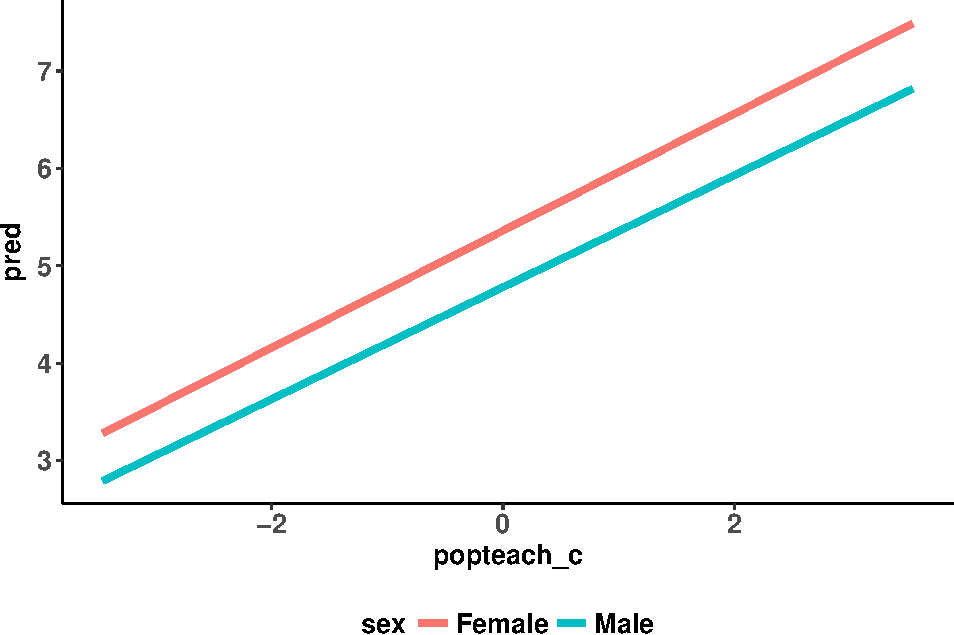
\includegraphics{Beck_HW_3_files/figure-latex/unnamed-chunk-2-1.pdf}

\section{Question 5}\label{question-5}

The parameter estimates and residuals can provide some very interesting
information for these data. See if you can figure out how to determine
answers to the following questions.

In general, once you have fit a model with lmer( ), the following
functions can be used to get various bits of information:

\texttt{resid(fit\_object)}: the Level 1 residuals (\(r_{ij}\))\\
\texttt{fitted(fit\_object)}: the predicted outcomes at Level 1
(\(Y_{ij}\))\\
\texttt{ranef(fit\_object)}: the Level 2 residuals (\(u_j\))\\
\texttt{fixef(fit\_object)}: the Level 2 fixed effects (\(\gamma\))\\
\texttt{coef(fit\_object)}: the Level 1 coefficients (\(\beta_j\))

For the following, identify the requested individual by class number
(and if relevant, by pupil number).

\subsection{Part A}\label{part-a-4}

Using the second model in Question 2, identify the teacher whose
popularity ratings were most highly related to peer-rated popularity
ratings. How high was that relationship?

\[popular_{ij} = \beta_{0} + \beta_1 * popteach\_c_{ij} + r_{ij}\]
\[\beta_0 = \gamma_{00} + u_{0j}\] \[\beta_1 = \gamma_{10} + u_{1j}\]

\begin{Shaded}
\begin{Highlighting}[]
\NormalTok{(raneffs <-}\StringTok{ }\KeywordTok{coef}\NormalTok{(mod1)[[}\DecValTok{1}\NormalTok{]] }\OperatorTok\StringTok{ }
\StringTok{  }\KeywordTok{data.frame}\NormalTok{() }\OperatorTok\StringTok{ }
\StringTok{  }\KeywordTok{mutate}\NormalTok{(}\DataTypeTok{class =} \KeywordTok{rownames}\NormalTok{(.)) }\OperatorTok
\StringTok{  }\NormalTok{tbl_df }\OperatorTok
\StringTok{  }\KeywordTok{arrange}\NormalTok{(}\KeywordTok{desc}\NormalTok{(}\KeywordTok{abs}\NormalTok{(popteach_c))))}
\end{Highlighting}
\end{Shaded}

\begin{verbatim}
## # A tibble: 100 x 3
##    X.Intercept. popteach_c class
##           <dbl>      <dbl> <chr>
##  1         2.68      0.792 82   
##  2         4.13      0.782 100  
##  3         4.18      0.776 48   
##  4         3.53      0.775 97   
##  5         4.00      0.772 8    
##  6         3.64      0.772 55   
##  7         4.30      0.771 31   
##  8         3.69      0.769 14   
##  9         4.00      0.766 86   
## 10         4.45      0.765 71   
## # ... with 90 more rows
\end{verbatim}

The strongest relationship between between teacher and peer popularity
ratings occurred in classroom \(82\),
\(\gamma_{10} + u_{1~82} = 0.7921922\).

\subsection{Part B}\label{part-b-4}

Using the model in Question 3, identify the teacher whose popularity
ratings were the least related to peer-rated popularity when compared to
what was expected for that teacher. How much poorer than expectation did
this teacher perform?\\
\[popular_{ij} = \beta_{0} + \beta_1 * popteach\_c_{ij} + r_{ij}\]
\[\beta_0 = \gamma_{00} + \gamma_{01}*gmc\_texp_j + \gamma_{02}*gmc\_mean\_pop\_t_j + u_{0j}\]\\
\[\beta_1 = \gamma_{10} + \gamma_{11}*gmc\_texp_j + \gamma_{12}*gmc\_mean\_pop\_t_j + u_{1j}\]

\begin{Shaded}
\begin{Highlighting}[]
\NormalTok{(s.teach <-}\StringTok{ }\NormalTok{broom}\OperatorTok{::}\KeywordTok{augment}\NormalTok{(mod2) }\OperatorTok\StringTok{ }
\StringTok{  }\KeywordTok{mutate}\NormalTok{(}\DataTypeTok{pupil =} \DecValTok{1}\OperatorTok{:}\KeywordTok{nrow}\NormalTok{(.)) }\OperatorTok\StringTok{ }
\StringTok{  }\KeywordTok{arrange}\NormalTok{(}\KeywordTok{desc}\NormalTok{(}\KeywordTok{abs}\NormalTok{(.resid))) }\OperatorTok\StringTok{ }
\StringTok{  }\NormalTok{tbl_df }\OperatorTok\StringTok{ }
\StringTok{  }\KeywordTok{select}\NormalTok{(popular}\OperatorTok{:}\NormalTok{.fixed, pupil)) }
\end{Highlighting}
\end{Shaded}

\begin{verbatim}
## # A tibble: 2,000 x 9
##    popular popteach_c gmc_texp gmc_mean_pop_t class .fitted .resid .fixed
##      <dbl>      <dbl>    <dbl>          <dbl> <int>   <dbl>  <dbl>  <dbl>
##  1    2.40     0.0526  - 2.26        -0.113      56    4.98  -2.58   5.00
##  2    8.40     0.550    10.7          0.389      62    5.87   2.53   5.85
##  3    3.30     1.48    -11.3         -0.537      60    5.69  -2.39   5.70
##  4    2.00    -1.06    - 1.26        -0.00494    89    4.28  -2.28   4.29
##  5    6.40    -0.391   - 1.26        -0.669      88    4.14   2.26   4.13
##  6    5.50     0.800    10.7          2.14       35    7.69  -2.19   7.72
##  7    3.80     0.294     7.74         0.645      29    5.94  -2.14   5.93
##  8    3.80     0.600   - 0.263        0.340      73    5.82  -2.02   5.84
##  9    7.70     1.17      1.74        -0.227      91    5.71   1.99   5.69
## 10    6.50    -1.47      5.74         0.410      68    4.51   1.99   4.49
## # ... with 1,990 more rows, and 1 more variable: pupil <int>
\end{verbatim}

\begin{Shaded}
\begin{Highlighting}[]
\CommentTok{# %>% group_by(class) %>% summarize(mean = mean(.resid)) %>% arrange(mean)}
\end{Highlighting}
\end{Shaded}

The weakest relationship between between teacher and peer popularity
ratings compared to expectation occurred in classroom \(56\),
\(Y_{ij} - \hat{Y}_{ij} = -2.58\).

\subsection{Part C}\label{part-c-3}

Using the Level 2 residuals from the model in Question 3, which class
exceeded their expected mean popularity the most? What was the simple
(OLS) mean popularity of this class? What was the empirical Bayes
estimate for the mean popularity of this class? Why are these two
estimates (OLS and EB) for this class's mean popularity different?

\[\beta_1 = \gamma_{10} + \gamma_{11}*gmc\_texp_j + \gamma_{12}*gmc\_mean\_pop\_t_j + u_{1j}\]

\begin{Shaded}
\begin{Highlighting}[]
\NormalTok{lm_fit <-}\StringTok{ }\ControlFlowTok{function}\NormalTok{(data) \{}
\NormalTok{  fit <-}\StringTok{ }\KeywordTok{lm}\NormalTok{(popular }\OperatorTok{~}\StringTok{ }\NormalTok{popteach_c, data)}
  \KeywordTok{t}\NormalTok{(}\KeywordTok{coef}\NormalTok{(fit)) }\OperatorTok\StringTok{ }\NormalTok{tbl_df }\OperatorTok\StringTok{ }\KeywordTok{setNames}\NormalTok{(}\KeywordTok{c}\NormalTok{(}\StringTok{"Intercept"}\NormalTok{, }\StringTok{"Slope"}\NormalTok{))}
\NormalTok{\}}

\NormalTok{ols_mods <-}\StringTok{ }\NormalTok{broom}\OperatorTok{::}\KeywordTok{augment}\NormalTok{(mod2) }\OperatorTok\StringTok{ }\NormalTok{tbl_df }\OperatorTok
\StringTok{  }\KeywordTok{arrange}\NormalTok{(}\KeywordTok{desc}\NormalTok{(.resid)) }\OperatorTok
\StringTok{  }\KeywordTok{group_by}\NormalTok{(class) }\OperatorTok
\StringTok{  }\KeywordTok{nest}\NormalTok{() }\OperatorTok
\StringTok{  }\KeywordTok{mutate}\NormalTok{(}\DataTypeTok{ols =} \KeywordTok{map}\NormalTok{(data, lm_fit))}

\NormalTok{raneffs <-}\StringTok{ }\KeywordTok{ranef}\NormalTok{(mod2, }\DataTypeTok{condVar=}\OtherTok{TRUE}\NormalTok{)}
\NormalTok{Coef    <-}\StringTok{ }\KeywordTok{as.matrix}\NormalTok{(}\KeywordTok{coef}\NormalTok{(mod2)}\OperatorTok{$}\NormalTok{class[}\DecValTok{1}\OperatorTok{:}\DecValTok{2}\NormalTok{])}
\CommentTok{# Then we select the posterior variances and covariances}
\CommentTok{# as an attribute and save it.}
\NormalTok{PVar <-}\StringTok{ }\KeywordTok{attr}\NormalTok{(raneffs[[}\DecValTok{1}\NormalTok{]], }\DataTypeTok{which =} \StringTok{"postVar"}\NormalTok{)}
\KeywordTok{dim}\NormalTok{(PVar) <-}\StringTok{ }\KeywordTok{c}\NormalTok{(}\DecValTok{2}\OperatorTok{*}\DecValTok{2}\NormalTok{ , }\DecValTok{100}\NormalTok{)}
\NormalTok{Coef_Var_Cov <-}\StringTok{ }\KeywordTok{t}\NormalTok{(PVar)}
\CommentTok{# And take it apart so each of the matrix elements for}
\CommentTok{# each school is a separate column.}

\NormalTok{L2_Resid <-}\StringTok{ }\KeywordTok{ranef}\NormalTok{(mod2)[[}\DecValTok{1}\NormalTok{]]}

\NormalTok{Coef <-}\StringTok{ }\KeywordTok{cbind}\NormalTok{(Coef,Coef_Var_Cov,L2_Resid)}

\CommentTok{# By_School <- ddply(HSB_Data, ~School, lm_fit)}
\CommentTok{# add to the Coef matrix and define as a dataframe.}
\NormalTok{Coef <-}\StringTok{ }\KeywordTok{bind_cols}\NormalTok{(Coef, ols_mods }\OperatorTok\StringTok{ }\KeywordTok{unnest}\NormalTok{(ols, }\DataTypeTok{.drop =}\NormalTok{ T)) }\OperatorTok\StringTok{ }
\StringTok{  }\KeywordTok{setNames}\NormalTok{(}\KeywordTok{c}\NormalTok{(}\StringTok{"EB_Intercept"}\NormalTok{,}\StringTok{"EB_Slope"}\NormalTok{,}\StringTok{"Intercept_Var"}\NormalTok{,}\StringTok{"Covariance"}\NormalTok{,}\StringTok{"Covariance_Too"}\NormalTok{,}
                 \StringTok{"Slope_Var"}\NormalTok{,}\StringTok{"Intercept_Res"}\NormalTok{,}\StringTok{"Slope_Res"}\NormalTok{,}\StringTok{"class"}\NormalTok{,}\StringTok{"OLS_Intercept"}\NormalTok{, }\StringTok{"OLS_Slope"}\NormalTok{)) }\OperatorTok
\StringTok{  }\KeywordTok{mutate}\NormalTok{(}\DataTypeTok{I_lwr =}\NormalTok{ EB_Intercept}\OperatorTok{-}\KeywordTok{sqrt}\NormalTok{(Intercept_Var)}\OperatorTok{*}\FloatTok{1.96}\NormalTok{, }
         \DataTypeTok{I_upr =}\NormalTok{ EB_Intercept}\OperatorTok{+}\KeywordTok{sqrt}\NormalTok{(Intercept_Var)}\OperatorTok{*}\FloatTok{1.96}\NormalTok{,}
         \DataTypeTok{S_lwr =}\NormalTok{ EB_Slope}\OperatorTok{-}\KeywordTok{sqrt}\NormalTok{(Slope_Var)}\OperatorTok{*}\FloatTok{1.96}\NormalTok{,}
         \DataTypeTok{S_upr =}\NormalTok{ EB_Slope}\OperatorTok{+}\KeywordTok{sqrt}\NormalTok{(Slope_Var)}\OperatorTok{*}\FloatTok{1.96}\NormalTok{) }
\end{Highlighting}
\end{Shaded}

Class \(62\) most exceeded their expected popularity by \(0.01\). The
simple (OLS) mean popularity of this class was \(5.71\) and the
empirical Bayes estimate was \(5.09\). These two estimate are different
because the MLM expected values leverage information about the
relationship between mean classroom popularlity and teaching experience.

\subsection{Part D}\label{part-d-3}

Using the model in Question 4, which kid (identify the class number and
kid number) exceeded expected popularity the most? What was that child's
actual peer-rated popularity?

\begin{Shaded}
\begin{Highlighting}[]
\NormalTok{(q5d <-}\StringTok{ }\NormalTok{broom}\OperatorTok{::}\KeywordTok{augment}\NormalTok{(mod3) }\OperatorTok\StringTok{ }
\StringTok{  }\KeywordTok{mutate}\NormalTok{(}\DataTypeTok{pupil =} \KeywordTok{as.numeric}\NormalTok{(}\KeywordTok{rownames}\NormalTok{(.))) }\OperatorTok\StringTok{ }
\StringTok{  }\NormalTok{tbl_df }\OperatorTok\StringTok{ }
\StringTok{  }\KeywordTok{arrange}\NormalTok{(}\KeywordTok{desc}\NormalTok{(.resid)))}
\end{Highlighting}
\end{Shaded}

\begin{verbatim}
## # A tibble: 2,000 x 14
##    popular  sex_c popteach_c class .fitted .resid .fixed   .mu .offset
##      <dbl>  <dbl>      <dbl> <int>   <dbl>  <dbl>  <dbl> <dbl>   <dbl>
##  1    8.40  0.495      0.550    62    6.30   2.10   5.69  6.30       0
##  2    6.00 -0.505     -0.550    27    3.95   2.05   4.46  3.95       0
##  3    8.40  0.495      1.91     46    6.43   1.97   6.51  6.43       0
##  4    6.60 -0.505     -1.71     29    4.74   1.86   3.80  4.74       0
##  5    7.40  0.495      1.79     48    5.63   1.77   6.44  5.63       0
##  6    6.50 -0.505     -1.47     68    4.73   1.77   3.93  4.73       0
##  7    4.90 -0.505     -1.20      2    3.13   1.77   4.09  3.13       0
##  8    5.30 -0.505     -1.87     99    3.58   1.72   3.71  3.58       0
##  9    7.40  0.495      0.857    70    5.72   1.68   5.87  5.72       0
## 10    7.70  0.495      1.17     91    6.04   1.66   6.06  6.04       0
## # ... with 1,990 more rows, and 5 more variables: .sqrtXwt <dbl>,
## #   .sqrtrwt <dbl>, .weights <dbl>, .wtres <dbl>, pupil <dbl>
\end{verbatim}

\begin{Shaded}
\begin{Highlighting}[]
\NormalTok{dat <-}\StringTok{ }\NormalTok{dat }\OperatorTok\StringTok{ }\KeywordTok{mutate}\NormalTok{(}\DataTypeTok{student =} \DecValTok{1}\OperatorTok{:}\KeywordTok{dim}\NormalTok{(dat)[}\DecValTok{1}\NormalTok{])}
\end{Highlighting}
\end{Shaded}

Student \(7\) in class \(62\) exceeded their expected popularity by
\(2.1\). Their rated popularity was \(8.4\).


\end{document}
